\documentclass{article}
\usepackage{main}

\title{Exercices de révision}
\author{Seconde 9}
\date{12 Mars 2025}

\begin{document}
\maketitle
\begin{center}
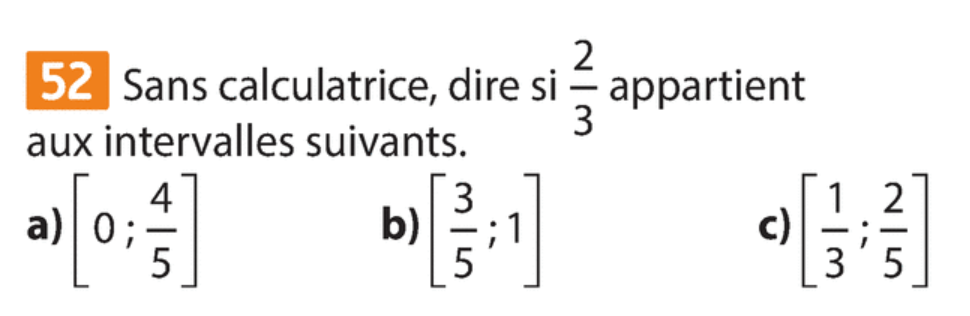
\includegraphics[width=\textwidth]{Exercice_1.png}
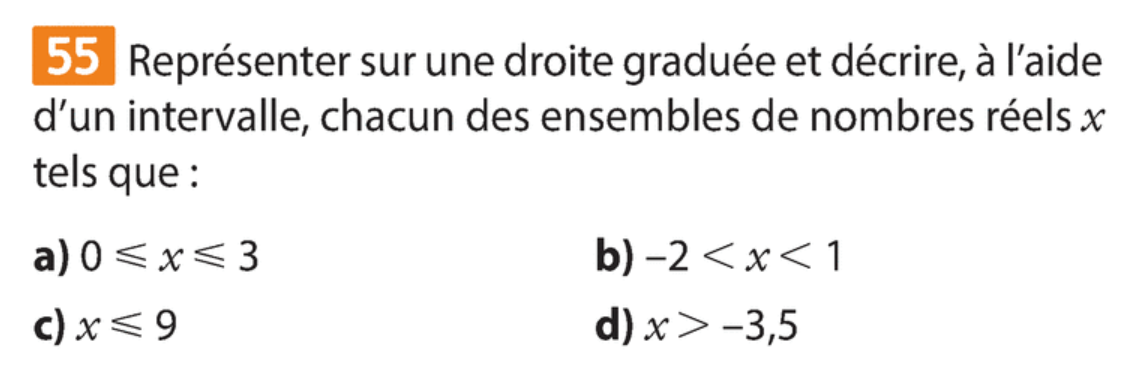
\includegraphics[width=\textwidth]{Exercice_2.png}
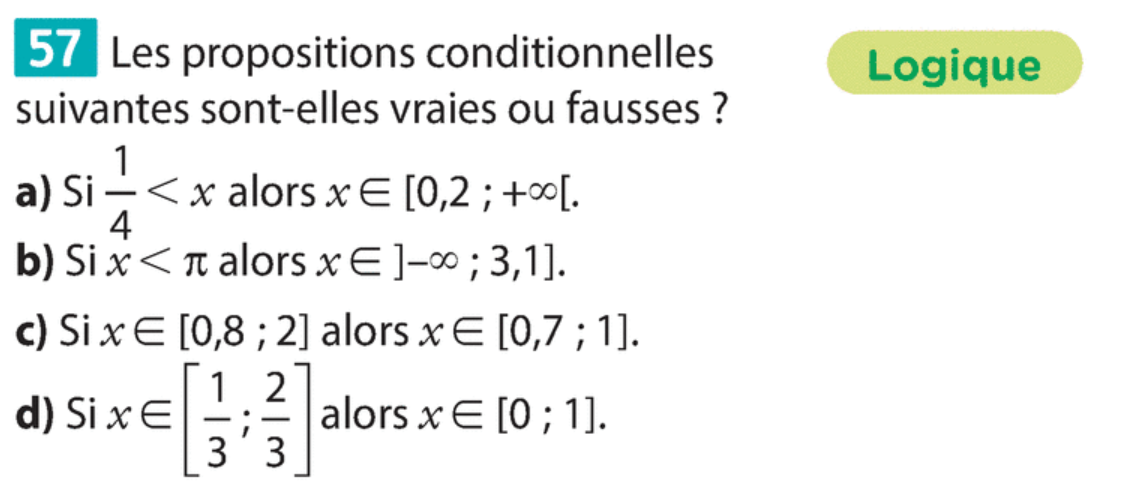
\includegraphics[width=\textwidth]{Exercice_3.png}
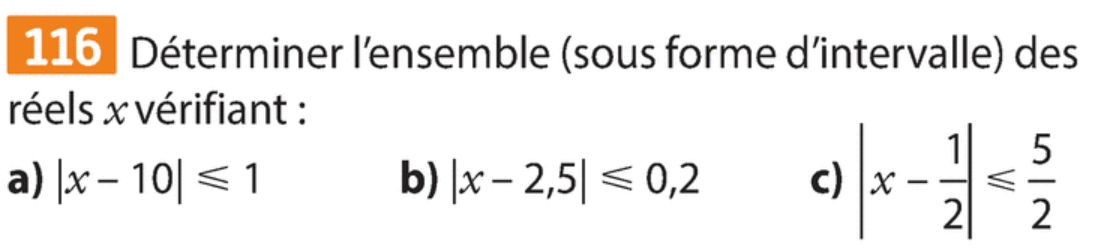
\includegraphics[width=\textwidth]{Exercice_4.png}
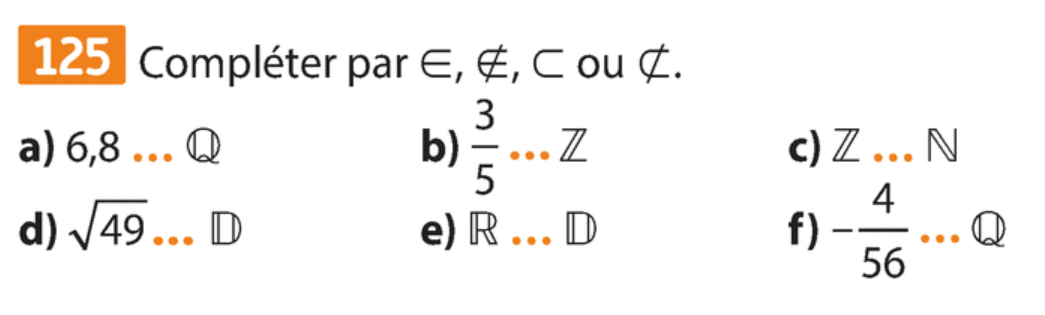
\includegraphics[width=\textwidth]{Exercice_5.png}
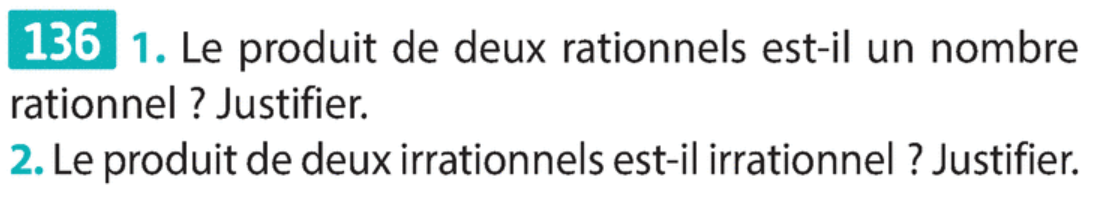
\includegraphics[width=\textwidth]{Exercice_6.png}
\vspace*{0.5cm}

\hrulefill

\vspace*{0.5cm}
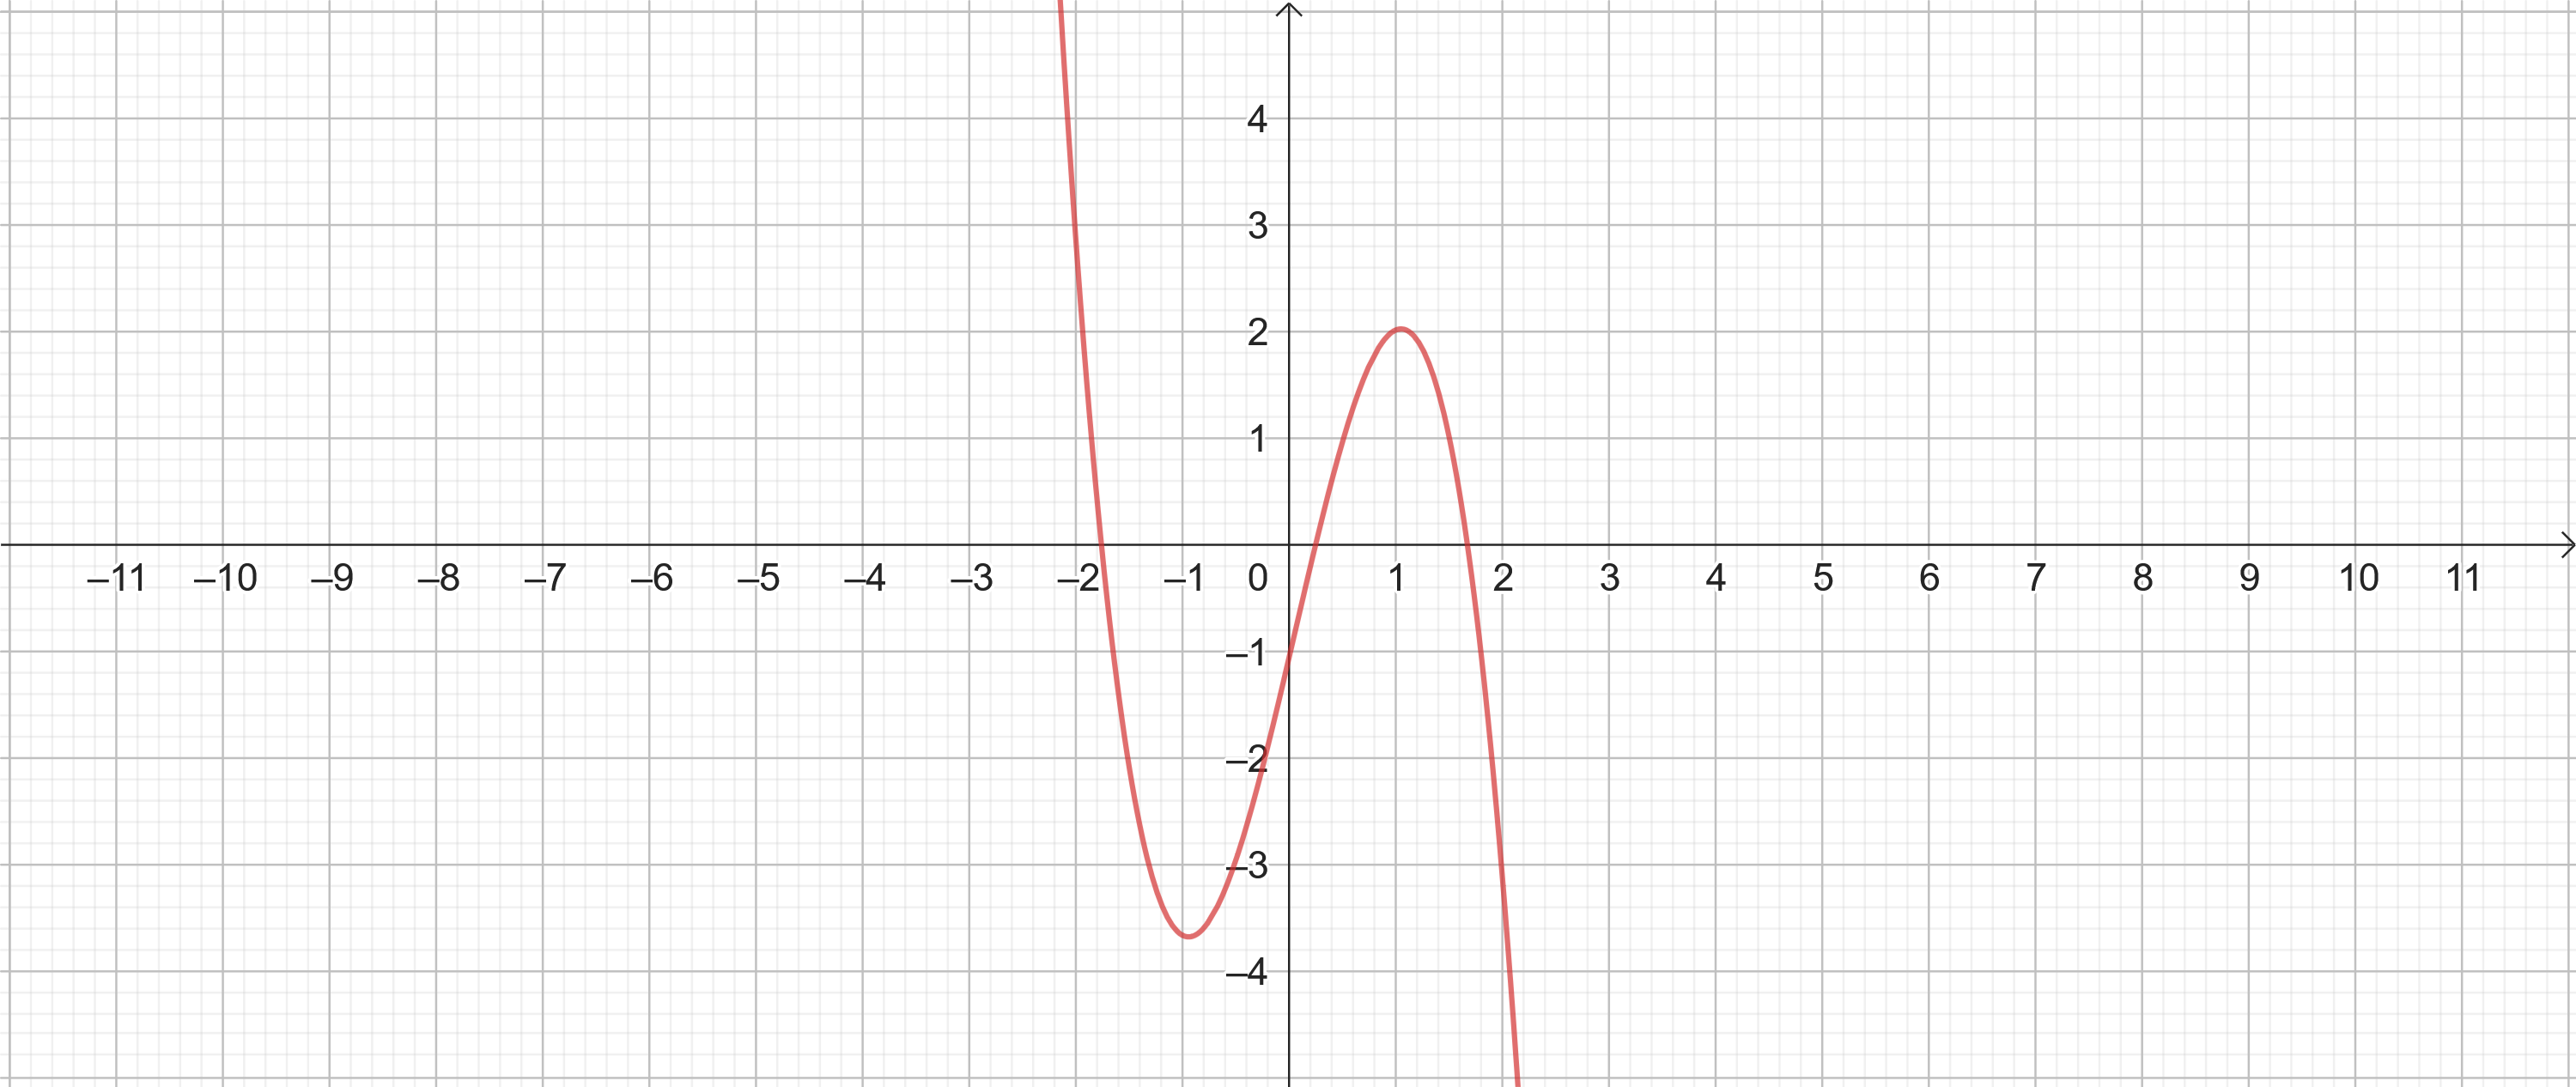
\includegraphics[width=\textwidth]{Exercice_7.png}
\end{center}
La courbe représentative d'une fonction $f$ est représenté sur le repère orthonormé ci-dessus.
\begin{enumquestions}
\item Quelle est l'image de $0$ par $f$ ? Et de $-2$ ?
\item Nommer deux antécédants de $-2$ par $f$.
\item Résoudre $f(x) > 1$.
\end{enumquestions}
\end{document}